%%%%%%%%%%%%%%%%%%%%%%%%%%%%%%%%%%%%%%%%%
% Short Sectioned Assignment
% LaTeX Template
% Version 1.0 (5/5/12)
%
% This template has been downloaded from:
% http://www.LaTeXTemplates.com
%
% Original author:
% Frits Wenneker (http://www.howtotex.com)
%
% License:
% CC BY-NC-SA 3.0 (http://creativecommons.org/licenses/by-nc-sa/3.0/)
%
%%%%%%%%%%%%%%%%%%%%%%%%%%%%%%%%%%%%%%%%%

%----------------------------------------------------------------------------------------
%	PACKAGES AND OTHER DOCUMENT CONFIGURATIONS
%----------------------------------------------------------------------------------------

\documentclass[paper=a4, fontsize=11pt]{scrartcl} % A4 paper and 11pt font size

\usepackage[T1]{fontenc} % Use 8-bit encoding that has 256 glyphs
\usepackage{fourier} % Use the Adobe Utopia font for the document - comment this line to return to the LaTeX default
\usepackage[english]{babel} % English language/hyphenation
\usepackage{amsmath,amsfonts,amsthm} % Math packages

\usepackage{lipsum} % Used for inserting dummy 'Lorem ipsum' text into the template
\usepackage{amsmath}
\usepackage{listings}
\usepackage{graphicx}
\usepackage{pdfpages}
\usepackage{enumerate}
\usepackage{color}
\usepackage{cite}
\usepackage{float}
\PassOptionsToPackage{hyphens}{url}\usepackage{hyperref}
\usepackage{sectsty} % Allows customizing section commands
\allsectionsfont{\centering \normalfont\scshape} % Make all sections centered, the default font and small caps
\usepackage[utf8]{inputenc}
\usepackage{fancyhdr} % Custom headers and footers
\pagestyle{fancyplain} % Makes all pages in the document conform to the custom headers and footers
\fancyhead{} % No page header - if you want one, create it in the same way as the footers below
\fancyfoot[L]{} % Empty left footer
\fancyfoot[C]{} % Empty center footer
\fancyfoot[R]{\thepage} % Page numbering for right footer
\renewcommand{\headrulewidth}{0pt} % Remove header underlines
\renewcommand{\footrulewidth}{0pt} % Remove footer underlines
\setlength{\headheight}{13.6pt} % Customize the height of the header

\usepackage{listings}
\usepackage{color}
 
\definecolor{codegreen}{rgb}{0,0.6,0}
\definecolor{codegray}{rgb}{0.5,0.5,0.5}
\definecolor{codepurple}{rgb}{0.58,0,0.82}
\definecolor{backcolour}{rgb}{0.95,0.95,0.92}
 
\lstdefinestyle{mystyle}{
    backgroundcolor=\color{backcolour},   
    commentstyle=\color{codegreen},
    keywordstyle=\color{magenta},
    numberstyle=\tiny\color{codegray},
    stringstyle=\color{codepurple},
    basicstyle=\footnotesize,
    breakatwhitespace=false,         
    breaklines=true,                 
    captionpos=b,                    
    keepspaces=true,                 
    numbers=left,                    
    numbersep=5pt,                  
    showspaces=false,                
    showstringspaces=false,
    showtabs=false,                  
    tabsize=2
}
 
\lstset{style=mystyle}


\numberwithin{equation}{section} % Number equations within sections (i.e. 1.1, 1.2, 2.1, 2.2 instead of 1, 2, 3, 4)
\numberwithin{figure}{section} % Number figures within sections (i.e. 1.1, 1.2, 2.1, 2.2 instead of 1, 2, 3, 4)
\numberwithin{table}{section} % Number tables within sections (i.e. 1.1, 1.2, 2.1, 2.2 instead of 1, 2, 3, 4)

\setlength\parindent{0pt} % Removes all indentation from paragraphs - comment this line for an assignment with lots of text

%----------------------------------------------------------------------------------------
%	TITLE SECTION
%----------------------------------------------------------------------------------------

\newcommand{\horrule}[1]{\rule{\linewidth}{#1}} % Create horizontal rule command with 1 argument of height

\title{	
\normalfont \normalsize 
\textsc{Copenhagen University, Bachalor Project - 2017} \\ [25pt] % Your university, school and/or department name(s)
\horrule{0.5pt} \\[0.4cm] % Thin top horizontal rule
\huge A blockchain implementation \\ % The assignment title
\horrule{2pt} \\[0.5cm] % Thick bottom horizontal rule
}

\author{Christopher Mulvad Groot - QZM830} % Your name

\date{\normalsize\today} % Today's date or a custom date

\begin{document}

\maketitle % Print the title
\thispagestyle{empty}
\newpage
\tableofcontents
\thispagestyle{empty}
\newpage

\clearpage
\setcounter{page}{1}

%----------------------------------------------------------------------------------------
%	PROBLEM 1
%----------------------------------------------------------------------------------------
\section{Abstract}

This reports seeks to gain a better and further understanding of blockchain technology, by researching and discussing the current uses and by deconstructing the blockchain, analyzing and explaining each part. Then an blockchain system is implemented in \texttt{haskell}, with working consensus mechanism, and the implementation is described and shown on a programmer level. Last but not least is an short discussion about the possibilities of blockchain structures replacing currently centralized systems, which to some extend could benefit from the blockchain approach. 

\section{Introduction}

For many, many years our societies have relied on institutions such as banks, governments and other centralized firms and businesses to keep track of everything from legal papers to money transactions. While modern time has demanded digitalization, in both public as well as private institutions with regards to ways of handling data, saving data and exchanging data, we find that it is often based on the idea of centralized system handling both regarding the adaptation of data as well as the verification. This require that the people relying on these services not only trust the systems handling their affairs, but also on the people who manage and owns the concerned systems. Another side effect of these centralized systems could be the complications that arises when moving any kind of data from one centralized system to another, which often results in long waiting time and a rather costly transaction fee.

\section{The Problem}

As a possible solutions to these previously mentioned and troublesome problems comes the blockchain system. I will in this project seek to gain a further understanding of the system and especially its consensus algorithms, especially the \textit{proof of work}, by making a simple implementation of a blockchain system. By this implementation I want to establish whenever a blockchain system would be protected from not validated modifications, and implementation-wise simple enough to qualify as a realistic replacement to todays data-storage. 

\subsection{Thesis}

Is the blockchain structure, complete with a working consensus mechanism, simple enough to understand and implement without any prior knowledge or experience with similar system structures. Or is such an implementation a rather complicated and time consuming process, requiring further research and understanding.

\section{Blockchain definition}
\label{sec:bcdef}

Now before diving into this report, the thoughts, work and implementation, I would like to define what in this report is understood as a complete blockchain system. As no precise definition is agreed upon among all blockchain enthusiast and as the creators hasn't stood up and declared the full meaning of term\cite{blockchainDef}. I will take the liberty of defining, at least in this humble writers perspective, what a blockchain has to contain to truly call itself a blockchain. When the word \textit{blockchain} in this report is used to describe a system it is expected to contain the following: 

\begin{enumerate}
\item \textbf{A distributed ledger}
\item \textbf{A block structure}, such as every piece of data points to the previous. 
\item \textbf{A consensus algorithm}, to ensure data integrity.
\end{enumerate}

Each part will be described further later in the  report.

\section{Data Handling Systems}

When talking about the blockchain way of constructing a system and its vast set of features, it is essential to highlight its most important trait, which alone has claimed the interest and enthusiasm from many people all around the world, it is of course the distributed ledger. Now the blockchain system isn't necessary the answers to all system designers prayers, as with any design choice it depends highly on the demands of the given system. However what it perhaps can do is replace currently centralized systems, like transactions systems in the financial sector or legal document storage in law firms or inside government. This is of course based on the assumption that a more open and inclusive system is wanted, expanding out of the boundaries of the centralized model and we will in this report not assumed otherwise. \\

To get a complete overview of the blockchain system features, possibilities and limitations one would first have to look at the system of which it should replace, the centralized systems.\\

\subsection{Centralized Systems}
Today many data handling systems are based upon the centralized system models, which is systems where the source code and, especially, the database is kept inside the same server system, in a single location. Thus when wanting to change and/or add new data and information one would have to connect to this, through local clients or network clients making it possible to access it from afar, while the data itself is still kept, saved and changed in one location. Having to accept the limitation and possible dangers of the system design. The type of dangers that a centralized system is prone to, as easier targets for hackers and even suffer minor inconveniences, such as data transportation both fourth and back between the main database, having to handle up to multiple clients. Even necessary precautions such as backup and DDOS attack prevention. Following figure \ref{fig:cenSys} illustrate how a centralized system could look like.

\begin{figure}[H]
  \caption{Centralized System}
  \centering
    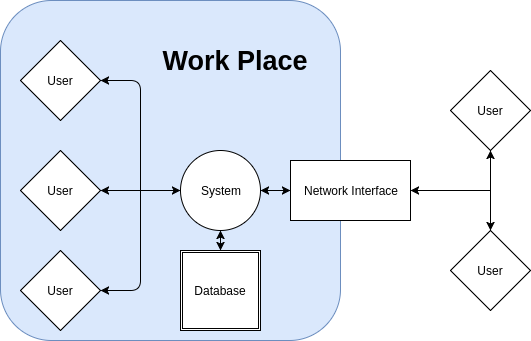
\includegraphics[width=0.5\textwidth]{CS.png}
  \label{fig:cenSys}	
\end{figure}

Now of course centralized systems have their benefits as well, as global data change for instance. Other advantages would be minimal data redundancy, as handling multiple copies of data can cause confusion and possible loss of the data's integrity\cite{centralized}. Data integrity and security seems to be hold in high regard in the centralized data model, however its biggest advantages ironically also contributes to its biggest disadvantages. With the perk of easy data change and addition comes also the fear of data tempering from possible illegal access, with a centralized database comes the obstacle of client traffic and so fourth\cite{compare}. It seems that to every advantage is an equal disadvantage, and while a centralized system can be an optional solution for some problems it certainly isn't for all. So to summarize:\\

\underline{Advantages:}

\begin{enumerate}
\item \textbf{Good data integrity} - only one main source.
\item \textbf{Minimum data redundancy} - only one copy.
\item \textbf{Easy data rewrite and change} - only one copy.
\item \textbf{High data security} - \textit{As long as the server is safe, then the data is as well.}
\item \textbf{High data accessibility} - no need to search multiple data storage facilities.
\end{enumerate}

\underline{Disadvantages:}
 
\begin{enumerate}
\item \textbf{Limited data connection} - as a centralized systems have to handle all pending connections itself. 
\item \textbf{Possible bottleneck\footnote{A bottleneck network is an condition in which the data flow is limited by the lack of network resources, as bandwidth\cite{bottleneck}}} - limited network resources can result in a network bottleneck.
\item \textbf{Possible data loss} - as data redundancy is at a minimum and the data itself is centralized it brings the danger of data loss.
\item \textbf{Total Control} - centralized systems also has the perk of being in total control over the data it processes, whenever this is a bad thing depends on the person. 
\end{enumerate}

\subsection{Decentralized Systems}

It is important to mention that decentralized systems in its own glory isn't a particular new invention. To take an example one could look at any other system build upon the \textit{Peer to Peer} architecture, especially many file-sharing systems are based upon this system architecture, projects like \textit{Napster}\footnote{Audio file sharing system\cite{napster}} and \textit{BitTorrent}\footnote{Used to share larger file between users\cite{bittorrent}}. The most important features of the \textit{Peer to Peer} system architecture are the opposite traits of a centralized system, instead having the users sharing resources, be it data, network bandwidth or process power among each other\cite{peer-to-peer}. Having data stored multiple places decreases possibilities of data loss as multiple copies exist, also having multiple client access point as user connect among themselves can prevent bottleneck collision. A distributed system based on the \textit{Peer To Peer} architecture can be seen in figure \ref{fig:peer} illustrated below.

\begin{figure}[H]
  \caption{Peer To Peer System }
  \centering
    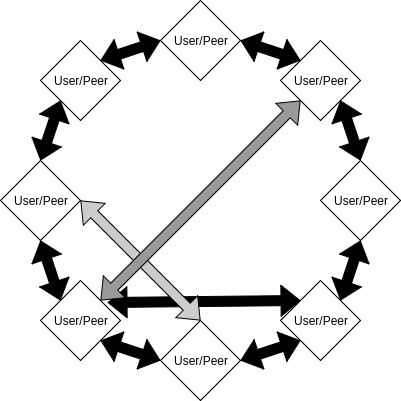
\includegraphics[width=0.5\textwidth]{p2p.png}
  \label{fig:peer}
\end{figure}

While this is an ideal solution for file sharing and the like, it as any other architecture have its limitation and disadvantage, with the limited centralization also meaning limited control over the system. This could be seen in some \textit{Peer to Peer} systems like \textit{Limewire} containing a high percentage of malware, nearly 63\% of executable or archive files contained some form of malware\cite{limestat}. This raises some suspicion towards the files integrity, if the file was possible to find, for to get a specific file from a peer the respected peer is required to be active thus in some cases limiting the data accessibility. Though some \textit{Peer to Peer} have successfully included peer and file protocols thus structuring their network and, to some extend, preventing malware and ensure data accessibility\cite{peer-to-peer}. However even with a structured system established we would still have a very high data redundancy which could prove a problem when trying to change or add data from a united standpoint. \\

As we can see that decentralized systems and especially \textit{Peer to Peer} architecture shows a lot of promise, however to be able to compete against a centralized system basis some feature addition have to be established. If all the users are expected to access and view the exact same data files, we have to ensure that all peers have access to the same data but still be able to uphold the decentralized system standard. Such a system would also need to be able to keep track of data, ensuring its integrity and protect it from being tempered with from any of the many peers\cite{distributed}. So to summarize the advantages and disadvantages of the \textit{Peer to Peer} based system:\\

\underline{Advantages:}

\begin{enumerate}
\item \textbf{High availability} - as the data usually can be find at more than one user.
\item \textbf{Less control} - depending on the system design it is possible to achieve a system demanding as little administration control as possible.
\item \textbf{Seldom data loss} - with high data redundancy follows the safety of declining data loss, as there exist multiple copies. 
\item \textbf{Multiple data connection} - as each user can act as an server, the possibility of running out of network bandwidth is less likely.  
\end{enumerate}

\underline{Disadvantages:}

\begin{enumerate}
\item \textbf{Complicated system design} - a decentralized system have to handle more unexpected problems and encounters, as it is moved out of the safe zone of a predefined hardware scenario and instead should handle custom setups.
\item \textbf{Hard to enforce data integrity} - with high redundancy comes, in this case, a lower data integrity.
\item \textbf{Complex database setup} - splitting a database over multiple nodes can become an advanced design challenge.
\item \textbf{Lower accessibility} - especially in unstructured \textit{Peer to Peer} designs, one would have to look among multiple sections of the system hoping to find data requested. 
\item \textbf{Hard to change data} - as the data is spread in copies over a larger network, it can be hard to press changes out to the whole system.
\end{enumerate}

\section{The Blockchain System}

Now with the generalized advantages and disadvantages listed on both typical centralized systems and distributed systems, here with focus on the \textit{Peer to Peer} approach, we can see that a vanilla\footnote{Term used to describe the basic form of a system. } \textit{Peer to Peer} systems still leave much to be desired. Such a system wouldn't live up to the main criteria set by the central system model, where especially factors such as control and data integrity weighs heavy. However as a possible solution comes the blockchain system approach with the promise of an including and secure way of storing and controlling data. To shorty describe the blockchain system approach, one can start by looking into the describing word itself.

\subsection{Block \& Chain}

The \textbf{block} describes the data structure as each piece of data is included into a block, or list if you will, which in addition to the original pierce of data holds other segments of information concerning the stored data which is deemed important by the developer. This could be information like the data creation timestamp, block number, name of block creator and, more importantly, the hash or the link to the previously block but more on that later. So in short it is a way to handle and describe your data such that all necessary information regarding each data is saved and accessible\cite{block}, this is typically denoted as a \textit{datatype}, below is in figure \ref{fig:bd} an block example illustrated.  

\begin{figure}[H]
  \caption{Block datatype}
  \centering
    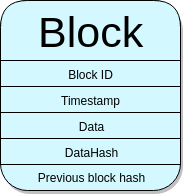
\includegraphics[width=0.35\textwidth]{block.png}
  \label{fig:bd}
\end{figure}

The \textbf{chain} describes the linked connection between the blocks, where each block always refer to the block before it creating a bond, or chain if you will, which holds the whole ledger together. Now a chain is only as strong as it weakest link and one of the strong selling points of the blockchain structure is keeping a high data integrity, so in order to keep an strong unchangeable data chain each link would have to be break resistance. Here the consensus algorithm is what a ordinary rust treatment would be to a metal chain, this is done by agreeing to some sort of specific procedure, or problem, that can be verified easily by the other peers\cite{consensus}. An illustration of such a chain can be seen below in figure \ref{fig:chain}.\\

\begin{figure}[H]
  \caption{The Chain}
  \centering
    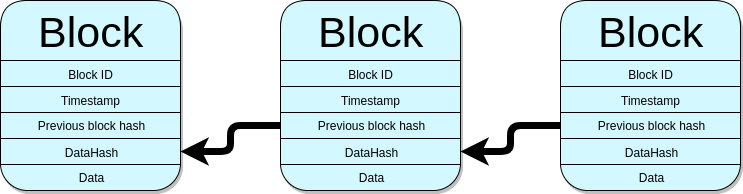
\includegraphics[width=1\textwidth]{chain.png}
  \label{fig:chain}
\end{figure}

To elaborate further on the subject of consensus mechanisms, we will in the following subsections dive into the other important aspects of this distributed system architecture.


\subsection{The Distributed Ledger}

The distributed ledger is the backbone of blockchains, every blockchain contains one as a ledger is needed for a network to be able to work from a united information point. The benefits of a ledger is well known and uses is dating back centuries, making it digital has further improved its uses, the next step would be the distribution. As we previously have mentioned some of the shortcomings of the distributed systems in its simple state, the distributed ledger can be the answer to some of the challenges. A problem was a declined data accessibility, as in the vanilla \textit{Peer to Peer} system some data may exclusive be available at some peers and not at others, which could result in a search for a online peer holding the desired data. Some peers might even hold an outdated version of the requested data, which makes it hard to refer to specific data and try to create universal changes. Here a distributed ledger creates a data baseline for all the peers, by relying on a ledger and holding it updated throughout the network the data accessibility is strongly increased\cite{ledger}. An illustrate of the main differences between the decentralized and distributed systems can be seen in figure \ref{fig:decen} below: 

\begin{figure}[H]
  \caption{Decentralized and Distributed}
  \centering
    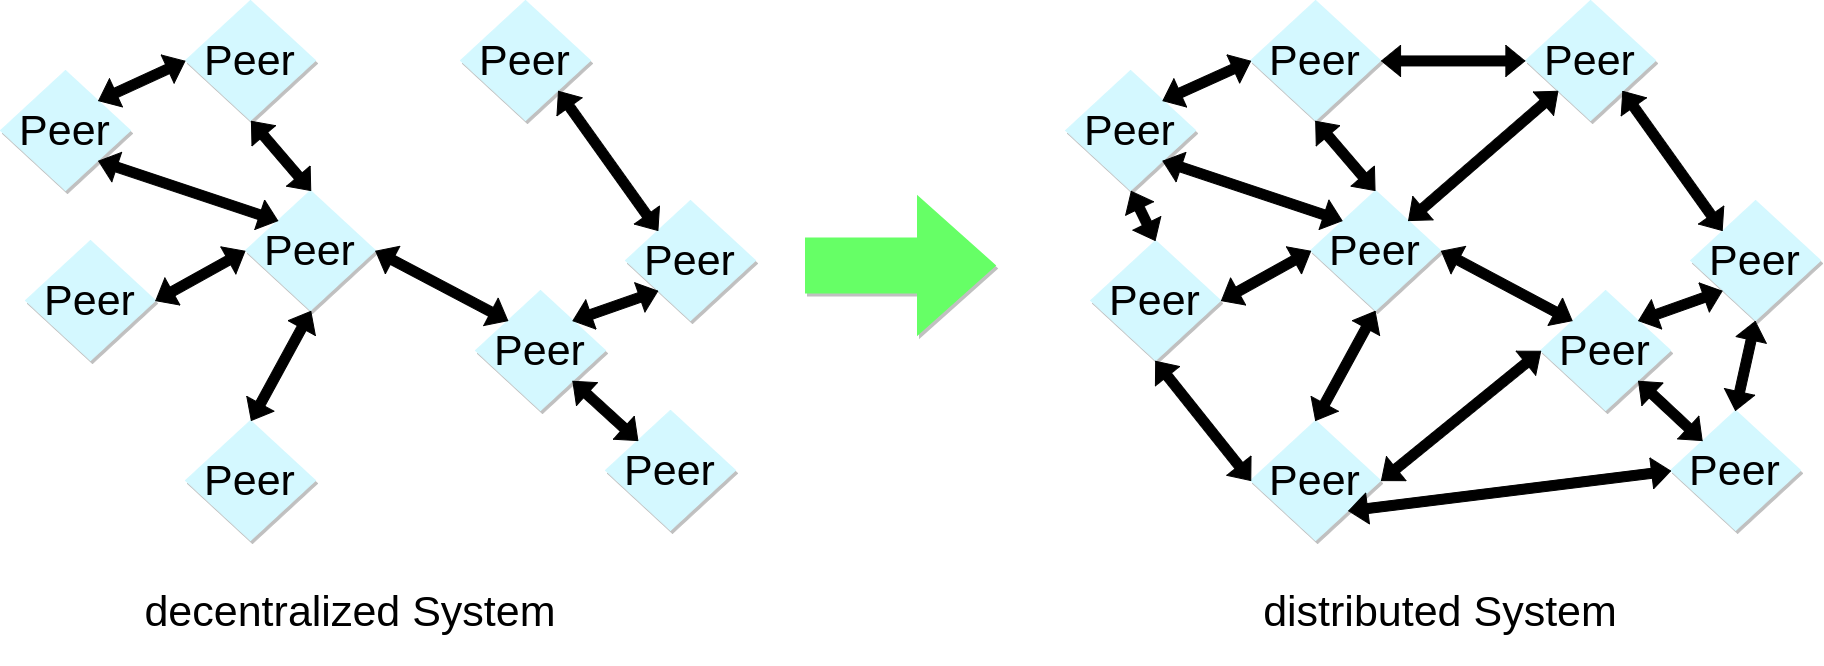
\includegraphics[width=1\textwidth]{centri.png}
  \label{fig:decen}  
\end{figure}
 
By distributing the system among the peers of the network, more tightly system changes and additions should be easier as all can operate from the same information baseline. Of course this raises the question how do one ensure that the whole network makes changes and addition based on the correct system version, how do one handle misinformation or even harmful wrong information around the network. To these challenges come along another feature of the blockchain, namely consensus mechanism. 

\subsection{Consensus algorithms}

Now the consensus mechanics play a big part in the blockchain, as it is a way to keep and ensure data integrity which otherwise would be hard to keep minding the distributed ledger. By the use of an consensus method the peers can between themselves agree, or give consent, to new changes made to the distributed ledger. Now different consensus approaches exists, each with their possibilities and limitations however each and every consensus mechanics must be fault tolerant or resilient\cite{consensus}. What is meant by this is that such a consensus mechanisme must be able to withstand or at least quickly recover in the event of a system fault, be it user or system wise. When talking about distributed systems faults one specific type is essential to be able to handle, the ones classified as \textit{Byzantine faults}. It is a type of faults most commonly associated with distributed computer systems, famously based on the \textit{ Byzantine Generals' Problem}\cite{byzan}. In short it concerns the problems and misunderstandings that can arise with the use of long communications, in a big network not all can be guaranteed the same information at the same time. There may be miscommunication between two peers resulting in wrong information being given, or a peer may deliberately be trying to spread false information. While it is impossible to ensure these problems don't arise\cite{general}, it is however possible to tolerate them by agreeing on a set of predefined rules which enables the distributed system to reach agreement despite faulty communications. A system able to handle these kind of faults is known to have a high \textit{Byzantine Fault Tolerance} (BFT), as a blockchain include a consensus mechanism these kinds of systems are known to be highly tolerant of Byzantine faults\cite{byzan}.  \\

As there are different ways of handling these kind of faults, we will be looking at two most well-known blockchain consensus mechanism. The highly used \textit{Proof of Work} method and the more complex but highly regarded \textit{Proof Of Stake}. 

\subsubsection{Proof of Work}

The \textit{Proof of Work} consensus mechanism is the most known of the two, given it is used \textit{bitcoin} structure. While not exactly a new invention, as its use is dated back to 1993, the idea to use it alongside a distributed system is\cite{proof}. The central idea behind this consensus mechanism is, as the name implies, the ability to proof that a type of work have been done and in a manner can be legitimatized. So the first part is to defined a certain task or problem that have to be solved in order to add a block to the surrounding chain, this is typically done with the help of cryptographic technology which if specified more leads us to the use of hashing, in this case that of \texttt{SHA256}. Now as SHA hashing is deterministic, it is a way of adding a unique, or seemingly\footnote{Collisions denotes the event of two different data files having the same hash\cite{collision}}, fingerprint to any kind of data defined in 1 and 0's, when hashing a string of, lets say "\texttt{hello world!}", it gives us an specific string, a hash. This hash is uniquely based on the piece of data it is given and will always return the same hash when feed the same data. Should any addition or changed to this piece of data be made, any shifts of bytes, then so will the hash associated with the string. The SHA-2 hashing produces a seemingly random string based on the information given, thus the approach to find the information behind a hash is typically performed by using brute force methods, thus SHA-2 provides some security qualifying it to be the hash chosen in blockchains like bitcoin\cite{sha}. The use of the shorter and more simple hash SHA-1 can be seen illustrated in figure \ref{fig:hash} below, noticed how a slight change such as changing the two letters "H" and "W" from upper-case to lower-case drastically changes the hash calculated.

\begin{figure}[H]
  \caption{SHA-1 Hashing}
  \centering
    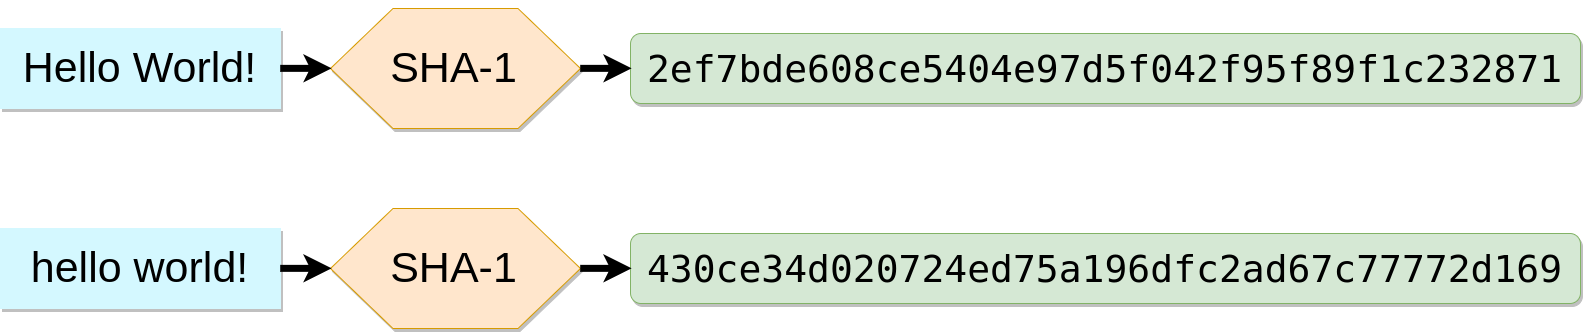
\includegraphics[width=1\textwidth]{hash.png}
  \label{fig:hash}
\end{figure}

With the use of this hashing technology, we can defined a specific problem or task to be solved when adding blocks to the chain. One could be that first \texttt{n} characters of the hash of the new block matches the last \texttt{n} characters of the previous block. However as the SHA hash seems randomly given how do we ensure that our new block, and the data within, satisfies this new task.\\

This process is denoted by the masses as \textit{Mining} and the name is fairly descriptive. As one can't foresee the SHA hash that's going to be given one would have to "try" their way into matching the desired hash, as adding simple data changes the whole hash this process can be done by keeping adding a number to the data until the desired hash is achieved. This number added is referred to as an \textit{Nonce} and is a number addition to the data that yields the preferred hash\cite{nonce}. As the suiting \textit{Nonce} can't be predicted one would have use brute force to find the correct \textit{Nonce}, thus costing energy resources used to calculate and find the hash which can be seen as the work done. Now while it does take work, resources and time to produce the hash it is fairly easy to verify. Each peer can simply calculate the hash themselves and see that it fulfills the task, thus proving that the work was done and the peer can then accept the new changes with peace in mind. An simplified illustration of the mining process can be seen in figure \ref{fig:mining} below:

\begin{figure}[H]
  \caption{Mining}
  \centering
    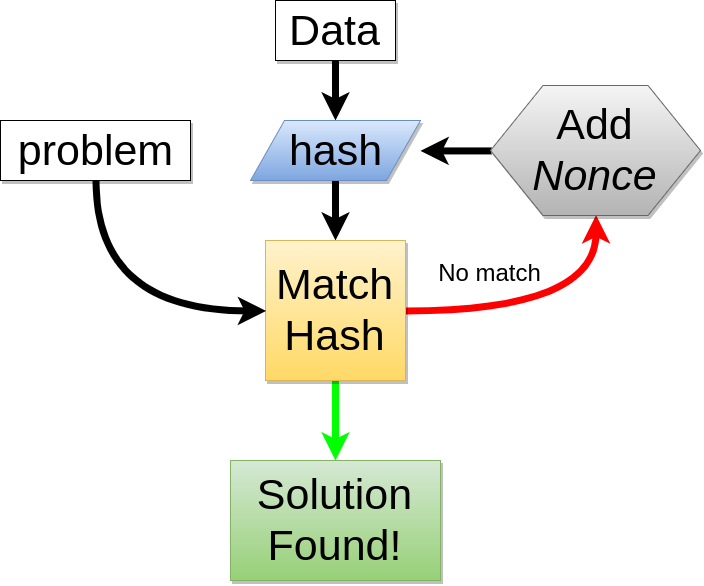
\includegraphics[width=0.5\textwidth]{mining.png}
  \label{fig:mining}
\end{figure}

Now this approach does satisfy some demands but have also been criticized for some of the others design choices. A big part of the \textit{Proof of Work} approach is that some users actually do the mining process, and as this cost both time and resources they must be given a reward. In the bitcoin model for example, the miners are given an amount of bitcoins as rewards where the amount is defined at the systems core. However as these coins appear out of thin air, thus becoming an addition to the whole bitcoin economy, the system slowly decreases the reward amount in fear of inflation\cite{mining}. It will then, at some point, reach a level where the reward does not simply equal the work cost, now what is proposed in the bitcoin system is that each miner is payed some transaction fee. This does however reach some new problems that is normally associated with the free market.\\

 A major possible flaw with this consensus mechanism is that the high computation cost might result in miners collaborating in mining firms if you will. Now if such an mining firms would consist of over 51\% peers of the entire network they would consensus vice be able to declined legitimate addition to the block chain, thus invalidating new blocks coming from the rest of network. While they wouldn't be able to make changes to previous blocks in the blockchain they would however be able to halt new blocks and transactions coming from around the network, controlling the flow if just for a short while. This may not be devastating to the distributed system but can cause some harm, of course to be in control of 51\% of the users on such a big network as the bitcoin network is unlikely, but not impossible\cite{51}. Another side effect of this consensus mechanism is the high energy cost, that follows from the mass computations needed during the work to compute the desired hash. This can have some environmental effect, which should be taken in to consideration when choosing a consensus mechanism.

\subsubsection{Proof of Stake}

This type of consensus method is created as a responds to the \textit{Proof of Work} consensus mechanism, so its uses have mainly been tied with digital currency systems. Now while it may not be limited to economic systems, we will only see the consensus mechanism in that kind of scenario, as it is the most common use and thus widely documented. \\ 

The \textit{Proof of Stake} consensus mechanism seeks to fix some of the shortcomings of the \textit{Proof of Work} approach. One of the highlighted points of this consensus mechanism is to get around the highly energy costing hashing calculations, by instead of having miners compete for the block rather follows a specific procedure to choose a 'miner', typically named a minter in this case, by chance. While the smith or minter is chosen at pseudo-random there are set some factors into play, here namely the \textit{stake} plays a role in how likely a peer is to be chosen. The stake represent how invested the peer are in the distributed system, in the case of digital currency it is normally tied to the amount of the digital currency owned. As different approaches exists, we will focus on the approach used by the \textit{Nxt}\cite{nxt} cryptocurrency as it is widely recognized for its use of the \textit{Proof of Stake} consensus mechanism.\\

We will denote the block creatings process as forging in this case instead of mining, as such no hard work in that sense is performed, but rather a peer is chosen to forge a block. Whether a peer is chosen to be the smith of the current block depends on two things, one is chance and the second is their forging power. Now if we start by looking at the term forging power, it is a way of weighing the peers investments in the system, typically a higher investments means a higher forging power. With the Nxt approach as starting point, the fording power is calculated the following way:\cite{stake}

\begin{center}
$b_k = \frac{B_k}{B_1+...+B_k},\ k=1,...,N$
\end{center}

\begin{itemize}
\item $b_k$ - Forging power.
\item $B$ - Account balance.
\item $N$ - Number of forging accounts.
\end{itemize}

This is based on the assumption that all accounts are online and forging. A bigger stake hold would thus yield a larger forging power, and this comes to play in the next part.\\
To pick the next account giving the honor, and transaction fee, of forging the next block comes the change segment. 

\begin{center}
$k_0 = argmax\frac{b_j}{U_j},\ j \in \{1,...,N\}$
\end{center}

\begin{itemize}
\item $argmax$ - Returns the maximum value
\item $b_j$ - Forging Power
\item $N$ - Number of of forging accounts.
\item $U$ - Random variable with uniform distributed interval (0,1).
\end{itemize}

This is the core principle behind the \textit{Proof of Stake} consensus mechanism, further restrictions and demands can be set to achieve further equality. One is a timeout for the stake used, such that after an account has created a block the stake currently hold by the account becomes invalid in the next $n$ timelimit, giving a brief chance for other accounts to weigh in.\\

This consensus mechanism is more energy efficient, as the miners, or forgers, does not have to show a specific solution to a hard problem, but rather just have to prove they are the owners of a specific stake. This could also provide a safer network, protecting against 51\% attacks, for while an miner would be able to buy expensive hardware and musscle their way in the same approach dosen't work with \textit{Proof of Stake}. While a miner can buy gear or get an advantage from outside the system, to get the upper hand of a \textit{Proof of Stake} network one would have to invest time and money into the system to get a significant enough stake. 

\subsection{Strength and weaknesses}

Now as we have gone through the different aspects of the blockchain system model, it is clear that while it does come closer towards a perfect decentralized system, with both a distributed ledger and consensus mechanism to back it up, it still have some flaws. As mentioned in the previous sections regarding the blockchain system, new problems arise from the ashes of beaten challenges. With the system initial intention to distribute both the system and the control to network, we are faced with the challenge of possible hostile takeover\footnote{51\% attack\cite{51}} which could revert the system back to centralized decision making. With a specific group of people on the top making addition to the ledger without the need of consent from the additional 49\% users.\\

Minding the \textit{Proof of Stack} consensus method as an alternative, we still face the challenge of the great energy consumption using cryptographic mining. With \textit{Proof of Work} still being the most recognized consensus mechanism regarding blockchain, high energy cost resulting in environmental damage still needs a more permanent solution. While \textit{Proof of Stack} could be a step on the way it still is a problem needing a substantial solution, keeping both energy cost down and the blockchain security at an all time high. To create an easier overview of the blockchain dis- and advantage, we will summarize them in the following two lists:\\

\underline{Advantages:}
\begin{enumerate}
\item \textbf{High availability} - as the same distributed ledger can be found all over the network.
\item \textbf{Seldom data loss}
\item \textbf{High data integrity} - thanks to the consensus mechanism.
\item \textbf{Durable system structure} - As the data is spread, an attack against the system would mean an attack against the whole network. 
\item \textbf{Easier data addition} - With the distributed ledger as the systems core, we have a structured system without the administration.
\item \textbf{Trust less system} - Peers don't need to trust each other but can rely on the consensus mechanism.
\item \textbf{Fast transactions}- Transaction of data is made easier as the whole network is connected together theres no need for slow system to system data transactions. 
\end{enumerate}

\underline{Disadvantages:}
\begin{enumerate}
\item \textbf{Complex system} - Playing with distributed solution raises some challenges implementation wise, while not unresolvable they can prove problematic.
\item \textbf{Energy cost} - While especially targeting the \textit{Proof of Work} method, we face a lot of computer computations.
\item \textbf{Require system transition} - While the blockchain is in many ways revolutionary, it is however a solution that don't meet halfway. A half decentralized centralized solution isn't necessarily the best of both worlds.
\end{enumerate}

\subsection{Blockchain possibilities}

When talking about the blockchain structure and features, most talk quickly leads to cryptocurrency or to some similar economic subject. While the blockchain does a good job of keeping track of currency transactions, it is merely the tip of the iceberg, the possibilities of the blockchain are vast and the purposes many. We will shortly go through some of them as to widen the perspective of the blockchain and to see it for the true possibilities it represent, instead of just being a synonym for BitCoin.\\

The most obvious uses is found inside the financial sector, with the possible replacement of centralized bank systems and instead one big blockchain. This would erase slow and costly money transactions between banks and thus tighten to world economy more closely, including everyone with some asset, a computer and a network connection. As each person can operate without the need of exchanging personal information normally needed to open a bank account, without the need of legal papers. This gives especially countries without proper population notation and structure the possibility to participate in the world economy. It also eliminates the needed trust, or distrust, to the world banks as the data can't be altered by a single network node, or most likely can't\cite{51}.\\

Cloud service is a useful way to preserve data, without the need for the everyday person to invest in extensive and expensive backup gear. Services such as google, microsoft and apple offers to hold and keep your data safe, however can one trust these companies to hold the data safe and sound from preying eyes. \textit{Storj}\footnote{Further information can be found at: \url{https://storj.io/}} is working on a distributed alternative, based on blockchain technology and offers users a way to safely and anonymously store data using data splitting and encryption to ensure data security. This should yield a more secure and stabel cloud service, without the need to comply to companies terms and conditions\cite{uses}.\\

In short blockchain can be a welcome solution in any sceneario where shared information is desired, it could be use to share passport information worldwide or to keep track of legal papers and their version, sign date and so on. Now the main reason these blockchain uses has been mentioned and shortly presented are that we must try to see the full range of possibilities that the blockchain can provide. If not, one can find themselves overwhelmed by some of the complex aspects of a big blockchain system, and despite the distributed system might provide a more safe and sustainable solution. The centralized system model is well tried and well documented and might prevent some developers from trying a new and less walked approach.


\section{Blockchain implementation}

In this section I will explain my design choices and challenges I faced during the implementation process. Simplicity was the key goal for this implementation, for as we looks towards big implementation like BitCoin with its vast selection of features it can be hard to separate the core blockchain and functions from addon componenets. Thus the main focus has been to try and limit the functionality to the most basic working blockchain, it will by intention lack some features introduced in larger blockchain implementation, though only non-core functions. The implementation will live up to the definition of a blockchain specified previously in this report\ref{sec:bcdef}. As there are many parts to this implementation i will focus on the program sections I find particular important.

\subsection{Expectations}

Before starting on the implementation I had some concerns about the consensus mechanism and expected it to be a implementational challenge, this was mainly due to the fact that I knew very little about it and what little I had heard did not explain how it worked or why it was secure enough to sustain systems holding complex implementation such as digital currency. Beside that I was also working with a completely new programming language as I hadn't previously worked with haskell, though i had some experience with different functional programming languages, such as ML.\\

The distributed network wasn't expected to prove such a challenge as it sooner turned out to be, this expectation was mainly based on the assumption that I could make a distributed network with few features, holding as few parts in play as possible. The \texttt{haskell} language was a kind of joker in this implementation plane, as i hadn't much interaction with it or had researched about it.

\subsection{Preset of implementation}
The implementation is programmed on/with the following systems used:

\begin{itemize}
\item \textbf{Programming Language:} - \textit{Haskell}
\item \textbf{System used:} - \textit{Ubuntu 16.04.2 LTS} 
\item \textbf{Compiler used:} - \textit{Glasgow Haskell Compiler, Version 7.10.3, stage 2 booted by GHC version 7.10.3}
\item \textbf{Text-editor used:} - \textit{Emacs v.24.5.1}
\end{itemize}

The following libraries is used in the implementation, and should be installed to ensure program stability.

\lstinputlisting[language=haskell, firstline=3, lastline=25]{../code/b1.hs}

\subsection{User guide}

This section will feature a short guide on how to run the program and further explain what commands are available. 

\subsubsection{Step-by-step}

The following step-by-step guide will explain how to set up two local servers connected to each other. How to establish a tcp client connection and add blocks to its local blockchain, then how share it across the network and how to update the local chain to that of the network. This guide is  fitted to be executed on a linux system.

\begin{enumerate}
\item Start up a new server with IP \texttt{127.0.0.1} and listening on tcp port\texttt{4000}.\\ In terminal write:  \texttt{"runhaskell b1.hs 4000 127.0.0.1"}
\item Start up a second server with IP \texttt{127.0.0.2} and listening on tcp port\texttt{4001} which connect to the previously launched server - \textit{To set up multiple servers follow same approach.}\\In terminal write: \texttt{"runhaskell b1.hs 4001 127.0.0.2 4000 127.0.0.1"}
\item Connect to first server as a tcp client.\\ in new terminal window write: \texttt{"telnet 127.0.0.1 4000"}\\
Type 'U' for user, follow same approach to connect user to the second server.
\item To add a piece of data to the clients local blockchain type 'bc add', and type the string when requested.\\ in client terminal window write: \texttt{"bc add"}, followed by the string to be stored.
\item To publish the chain type the following command in the client window.\\
in client terminal window write: \texttt{"bc broadcast"}.
\item In the second client window an update \textit{">> new blockchain is avaible"}, should have been received. To view this new chain type \texttt{pbc show}, and to update the current local blockchain to it type \texttt{bc update}.\\
in client terminal window write: \texttt{"bc update"}.
\item To quit the client connection type \texttt{quit} in the client window, this will not stop the server however, it has to be stopped manually.\\
in client terminal window write: \texttt{"quit"}.
\end{enumerate}

\subsubsection{List of commands:}

\begin{enumerate}
\item \textbf{quit} - Closes the current tcp connection.
\item \textbf{help} - The help command alone list the supported commands, it has further the following sub commands: 
\begin{itemize}
\item \textit{pbc} - Explain the pbc command.
\item \textit{bc} - Explain the bc command.
\item \textit{quit} - Explain the quit command.
\item \textit{bc} - Explain the bc command.
\end{itemize}
\item \textbf{bc} - The bc commands mainly concerns the blockchain currently hold by the tcp client, it has further the following sub commands: 
\begin{itemize}
\item \textit{add} - Begins the process of adding a string to the blockchain.
\item \textit{broadcast} - Broadcast the currently hold blockchain across the network
\item \textit{show} - Shows the currently hold blockchain inside the clients window.
\item \textit{update} - Updates the currently hold blockchain to the latest published chain.
\end{itemize}
\item \textbf{pbc} - Commands concern the latest publicized blockchain on the network. It has the following sub commands: 
\begin{itemize}
\item \textit{show} - Shows the latest published blockchain.
\end{itemize}
\end{enumerate}

\subsection{Data structure}

Now a major design choice is how to block struture is formed, for this i took inspiration from the block structure in the BitCoin system, however significantly simplified as my implementation doesn't have several major protocols. The block structure is defined below: 

\lstinputlisting[language=haskell, firstline=27, lastline=32]{../code/b1.hs}

As can be seen we have several parameters:
\begin{itemize}
\item \texttt{index} - Simply denotes the blocks number in the chain, is only used for visual purpose. 
\item \texttt{prehash} - Contains the previous block hash, thus linking it the previous block. 
\item \texttt{timestamp} - Contains the timestamp from the blocks creation, not necessarily from the time it was added to the chain. 
\item \texttt{bdata} - The data which is stored in the block, this is not hashed and is fully exposed.
\item \texttt{psol} - The solution to the consensus problem, a number which when added to the bdata satisfies the consensus mechanism.
\item \texttt{bhash} - The current hash of the data + psol. 
\end{itemize}

More parameter and information could be added to the structure, however by keeping it simple and neat future modification are easier made. This keeps the system as a nice and clean blockchain basis.

\subsection{Proof of work mechanism}

As the point of the implementation was to implement a fully functional blockchain, but still keep it as simple as possible the consensus mechanism was a delicate matter. How simple could I make it and still be able to call it a consensus mechanism. As \textit{Proof of Work} seemed like the most used, i choose this for implementation, the consensus mechanism is split up into multiple function and we will thus go through each of them.\\

Firstly to create the hash we use the following function called \texttt{hashblock}: 

\lstinputlisting[language=haskell, firstline=99, lastline=106]{../code/b1.hs}

Which takes the hash of the previous block, the current data to be hashed, and the start point for the psol number, usually 0. By the use of a sha hash library, the bdata and the current psol value is hashed together, the first $n$ characters of the hash is then extracted and compare to the $n$ last characters of the previous hash. Should these match then the hash and psol value is returned. If not then the psol value is increased until a matching hash is achieved. A global challenge number $n$ is at the start in the code, increasing this would mean a higher difficulty as more charecters should match. Higher difficulties could yield unexpected results as psol is a int and thus there is an number limit at $2^{29}-1$, thus it might not find a matching combinations. I did not however have time to research further into this matter and as such the hashing functions still stand as it is.\\

The next function \texttt{checkSolution} simply checks the work, thus validating and creating consensus about the addition to the chain: 

\lstinputlisting[language=haskell, firstline=56, lastline=67]{../code/b1.hs}

This functions takes the hash from the previous block, the data from the current block and the promised solution psol. It then simply hashes the data and solution anew, then compare it to the previous hash making sure it passes the requirement previously set. It then return its results in the form an boolean.\\
two more functions regarding work confirmation is the functions \texttt{checkChain} and \texttt{checkChain2} two half of a whole:

\lstinputlisting[language=haskell, firstline=70, lastline=96]{../code/b1.hs} 

This function automatize the confirmation process to a whole blockchain, thus by feeding it a blockchain it returns whenever the whole blockchain satisfies the challenges, in the process verifying the work.

\subsection{distributed system}

Many parts of the program, minor and major, juggles with different web sockets and threads process, i will thus focus on some parts of the program that seems more significant than others, the whole code is however available in the code folder.\\

While the \texttt{main} function does setup the socket connections, and additionally connects to other servers if specified, the more central function handle the incoming connections is the \texttt{runConn} function:

\lstinputlisting[language=haskell, firstline=296, lastline=345]{../code/b1.hs}

It takes as input the following: 
\begin{itemize}
\item \texttt{(sock,\_)} - Socket which it should handle
\item \texttt{chan} - The channel used for communications between Web sockets connections, \item \texttt{universalBC} - The variable holding the latest blockchain change
\item \texttt{msgNum} - The channel message number.  
\end{itemize}

First it establish the broadcasting channel, securing a communications line, then it handles the given socket establishing a connections. Then I have chosen to only use one tcp port as both server and user access point, this seemed like a good idea at first but it might give unforeseen complications should one continue with further development. After confirming the connection type, server or user, it then establish an reader in a new thread which reads from the communications line and, depending the connection type, takes an responding action.\\

Should it be an user and should the message contain a new blockchain it is then saved inside the thread secure variable universalBC, which seemed the only option to move datatypes between threads.\\

Should it instead be a server then the reader would react differently, instead broadcasting it back to the server from which it was send. Thus creating a way to distribute the blockchain between systems.


\subsection{Challenges during implementation}

As with all programming project complications are a natural part of the process, now there was some minor problems as an extend of the language syntax. These, while annoying, didn't prove to be too difficult to overcome and could be solved and learned by a trial and error approach.
Even the consensus mechanism didn't give too many problems, of course some time had to be invested into understanding and researching the algorithm. But eventually I feel it was possible to create a somewhat simple and understandable function while still upholding some data security.\\

Now where the biggest challenge hid itself was in the implementation of an distributed ledger, getting the system to connect through web sockets  and sending and receiving correct data. This proved a much, much greater task than anticipated but was eventually solved. The idea and principles behind the distributed ledger idea is more simple on paper than I felt it was in reality. Of course this is a strictly subjective opinion but other developers who have mainly been working with centralized systems might feel the same way. 

\subsection{Shortcomings}

The implementation isn't without flaws and while it should live up to the blockchain definition mentioned earlier\ref{sec:bcdef} some parts are most definitely improvable. Below are some improvable sections of the program worth mentioning:\\

\underline{\textbf{Not tested properly}}

I haven't written a test program to test and find unforeseen errors in the program as I couldn't quite see the best approach, if I had more time this would be the first task to workout.\\
\newpage
\underline{\textbf{Syntax hiccups}}

There are most likely some minor syntax hiccups that could be visually and maybe runtime wise improved, I fear my sudden transaction from object oriented programming to functional programming might have taken its toll.\\

\underline{\textbf{Only tested on local network}}

As all use of the system have been on a local network, thus more of emulation of a true distributed network, it should be able to translate over to user on a real network, maybe demanding some minor tweaks.\\

\underline{\textbf{No User Protocol}}

The system does not have any user protocol, thus not keeping track of who and where certain changes have been made, instead it focused on validating the work delivered not on what data is submitted and who submitted it. This might in some case show up as an shortcoming, but in reality it is about the system and the expected functionalities. The blockchain itself don't demands such protocols to work, thus making them removable in this implementation.\\

\underline{\textbf{No block queue}}

Systems like BitCoin have races as to who can mine the next block fastest, as competition mining is an important feature of this blockchain  based system, so is keeping the combative miners in line. This includes functions handling multiple blocks being mined at the same time and which to append to the overall blockchain, these features are nessecary in the BitCoin systems as there are rewards associated with the mining and the new blocks. In this implementation however there is no such reward system and thus no need was felt to implement such function, of course there is no forcing update function either. This means that whenever a client want to update their blockchain is purely voluntary and while the new blockchain is validated it is not checked if it are longer or newer. This can make it difficult to uphold the distributed ledger principle, which is an possible improvement point.  


\section{Is blockchain the future? - discussion}

Now as we have looked into the abilites and possitibilites the blockchain provides, while still looking crititcal on the disadvantage one question still stands, is it the best system approach. Of course we will in this dicussion not make the generalization that the blockchain structure is an overall better system structure, but rather discuss its usability in cases where an actual blockchain implementation is possible and maybe plausible. So when talking about replacing current centralized systems, we are referring to systems where an blockchain implementation would be a possible improvement, like money transactions systems, legal document storage systems etc.
\newpage
\subsection{What is in favor of it?}

We can start by mentioning the benefits of the blockchain system, which is mainly data accessibility while maintaining data integrity, and then the systems ability to withstands overturn attacks and falsely information. Data transfer and addition is also more easy and cheaper time and resource wise in contrast to having separated centralized systems each handling some part of a larger transaction system. This also provides a more inclusive system and each user only need access to one big systems instead of having to be verified for access in multiple systems.\\

There is less central administration and verification, less upkeep resources is needed and when first the system is up and running the users take over minimizing additional overseeing. Of course there are still need for some administration, as new blocks needs to be added and some transactions fees needs to be collected. This occupation could rightfully be given to the banks, which would still be able to collect some transactions fee and in the same instance ease the system transition for larger companies.  

\subsection{What goes against it?}

The most prominent barrier against the blockchain system is not only its complexity, but rather the change it brings and the many larger companies it threatens. While bigger blockchain projects does contain some challenges implementation wise, it is rather whenever the systems it is meant to, not replace, but improve would be willing to cooperate. It is a big shift in control over markets such as the financial sector, where an account in a centralized system would be replaced with an account in the new global network. This would mean some money loss for the companies in the line of fire, here the banks, which in addition to financial loss also would mean less control over peoples money and accounts.\\

If the current centrilized systems owners decide for a more open systems, there will of course be some challenges system design wise, which can result in high development cost. It would however be a temporary loss, as is all systems development process but it could scare minor companies from trying new approaches and systems.

\section{Conclusion}

Implementing a blockchain have taken some time to understand, and while it remains a simple implementation it was still possible to implement. So in short it is a yes to our original problem, but had it been a more feature full version of a blockchain as a kind of BitCoin model then it most likely wouldn't have been done and working in time. While it was possible to understand and work with a simplified blockchain there are still vast features and new abilities to explore with more and more coming each year. I don't think the full extend of the blockchain possibilities is reached yet, and when bigger companies or countries starts to use and build system based on blockchain or distributed ledger technology, then I think we will see a drastic raise in possible uses.  

\newpage

\begin{thebibliography}{9}
\addcontentsline{toc}{section}{References} 
\bibitem{simpleBlock} 
Judd Bagley:
\textit{What is Blockchain Technology? A Step-by-Step Guide For Beginners}. \\ \url{https://blockgeeks.com/guides/what-is-blockchain-technology/} \\Blockgeeks, Upload: Feb 13, 2017, Web: 6 June 2017 - 1:11 am.
 
\bibitem{centralized} 
Multiple Authors:
\textit{Centralized database}.\\
\url{https://en.wikipedia.org/wiki/Centralized_database}\\ 
Wikipedia, Upload: 20 January 2017, Web: 6 June 2017 - 1:20 am.

\bibitem{distributed} 
Multiple Authors:
\textit{Distributed database}.\\
\url{https://en.wikipedia.org/wiki/Distributed_database}\\ 
Wikipedia, Upload: 28 May 2017, Web: 6 June 2017 - 10:49pm.

\bibitem{peer-to-peer} 
Multiple Authors:
\textit{Peer-to-peer}.\\
\url{https://en.wikipedia.org/wiki/Peer-to-peer}\\ 
Wikipedia, Upload: 4 May 2017, Web: 6 June 2017 - 2:50 pm.

\bibitem{proof} 
Multiple Authors:
\textit{Peer-to-peer}.\\
\url{https://en.wikipedia.org/wiki/Proof-of-work_system}\\ 
Wikipedia, Upload: 26 April 2017, Web: 10 June 2017 - 3:05 pm.

\bibitem{consensus} 
Multiple Authors:
\textit{Consensus (computer science)}.\\
\url{https://en.wikipedia.org/wiki/Consensus_(computer_science)}\\ 
Wikipedia, Upload: 15 March 2017, Web: 9 June 2017 - 9:42 pm.

\bibitem{napster} 
Multiple Authors:
\textit{Napster}.\\
\url{https://en.wikipedia.org/wiki/Napster}\\ 
Wikipedia, Upload: 16 May 2017, Web: 6 June 2017 - 2:55 pm.

\bibitem{block} 
Multiple Authors:
\textit{Blockchain blocks}.\\
\url{https://en.bitcoin.it/wiki/Block}\\ 
Wikipedia, Upload: 4 march 2016, Web: 9 June 2017 - 8:19 pm.

\bibitem{bittorrent} 
Multiple Authors:
\textit{BitTorrent}.\\
\url{https://en.wikipedia.org/wiki/BitTorrent}\\ 
Wikipedia, Upload: 1 June 2017, Web: 6 June 2017 - 14:55 pm.
 
\bibitem{compare} 
Eric Dosal: \textit{Centralized vs Distributed Computing},
\\\url{http://www.compuquip.com/2009/11/20/centralized-vs-distributed-computing/}\\ Compuquip Technologies, Upload:
20 November 2009, Web: 6 June 2017 - 1:44 am. 

\newpage
\bibitem{blockchainDef}
Sebastien Meunier: \textit{Blockchain technology - a very special kind of Distributed Database} \\
\url{https://medium.com/@sbmeunier/blockchain-technology-a-very-special-kind-of-distributed-database-e63d00781118}\\
Medium, Upload: Dec 29 2016, Web: 6 June 2017 - 2:20 am.

\bibitem{limestat}
J. Goebel, T. Holz and C. Willems: \textit{Detection of Intrusions and Malware, and Vulnerability Assessment}(2007) - by B. M. Hämmerli, R. Sommer. Page 112 \\ ISBN: 9783540736134

\bibitem{bottleneck} 
\textit{Network Bottleneck},
\\\url{https://www.techopedia.com/definition/24819/network-bottleneck}\\ Techopedia - Web: 6 June 2017 - 5:17 pm.

\bibitem{consensus2} 
Paul Krzyzanowski:
\textit{Consensus}.\\
\url{https://www.cs.rutgers.edu/~pxk/417/notes/content/consensus.html}\\ 
PK.org, Last Update: 23 February 2017, Web: 10 June 2017 - 2:06 am.

\bibitem{byzan} 
Multiple Authors:
\textit{Byzantine fault tolerance}.\\
\url{https://en.wikipedia.org/wiki/Byzantine_fault_tolerance}\\ 
Wikipedia, Last Update: 27 May 2017, Web: 10 June 2017 - 2:18 am.

\bibitem{general} 
Alessandro Panconesi:
\textit{The coordinated attack and the jealous amazons}.\\
\url{http://wwwusers.di.uniroma1.it/~asd3/dispense/attack+amazons.pdf}\\ 
DSI - La Sapienza via Salaria 113, piano III
00198 Roma, Italy.\\ Web: 10 June 2017 - 2:50 am.

\bibitem{sha} 
Multiple Authors:
\textit{SHA-2}.\\
\url{https://en.wikipedia.org/wiki/SHA-2}\\ 
Wikipedia, Last Update: 5 June 2017, Web: 10 June 2017 - 3:57 am.

\bibitem{nonce} 
Multiple Authors:
\textit{Cryptographic nonce}.\\
\url{https://en.wikipedia.org/wiki/Cryptographic_nonce}\\ 
Wikipedia, Last Update: 25 March 2017, Web: 10 June 2017 - 12:34 am.

\bibitem{collision} 
M. Stevens, E. Bursztein, P. Karpman, A. Albertini, Y. Markov:
\textit{The first collision for full SHA-1}.\\
\url{http://marc-stevens.nl/research/papers/SBKAM17-SHAttered.pdf}\\ 
Google Research and CWI Amsterdam, accepted at Crypto 2017. \\Web: 10 June 2017 - 1:0 pm.

\bibitem{51} 
 Daniel Cawrey:
\textit{51\% Attack}.\\
\url{http://www.coindesk.com/51-attacks-real-threat-bitcoin/}\\ 
Coindesk. Last update: 20 June 2014, Web: 10 June 2017 - 2:10 pm.


\bibitem{mining} 
Multiple Authors:
\textit{Mining}.\\
\url{https://en.bitcoin.it/wiki/Mining}\\ 
Wikipedia. Last Update: 26 December 2016, Web: 10 June 2017 - 3:57 am.

\bibitem{nxt} 
Multiple Authors:
\textit{Nxt}.\\
\url{https://en.wikipedia.org/wiki/Nxt}\\
Wikipedia. Last Update: 10 June 2017, Web: 11 June 2017 - 3:13 am.

\bibitem{stake} 
Serguei Popov:
\textit{A Probabilistic Analysis of the Nxt Forging Algorithm}.\\
\url{http://www.ledgerjournal.org/ojs/index.php/ledger/article/view/46/60}\\
Ledger Journal, ISSN: 2379-5980. Published: 2016. Web: 11 June 2017 - 3:13 am.


\bibitem{uses} 
WeUseCoins:
\textit{Potential Uses of Blockchain Technology}.\\
\url{https://www.weusecoins.com/blockchain-uses/}\\
WeUseCoins.com. Upload: 1 April 2016, Web: 11 June 2017 - 4:18 am.

\bibitem{ledger} 
Matthew Hancock, Ed Vaizey:
\textit{Distributed Ledger Technology:
beyond block chain}.\\
\url{https://www.gov.uk/government/uploads/system/uploads/attachment_data/file/492972/gs-16-1-distributed-ledger-technology.pdf}\\ 
UK Government Chief Scientific Adviser - Last Update: 19 January 2016, Web: 10 June 2017 - 6:02 pm.

\end{thebibliography}
\end{document}